\documentclass[lualatex,aspectratio=169]{beamer}

\usepackage[utf8]{inputenc}
\usepackage[T1]{fontenc}
\usepackage{xspace}
\usepackage{graphicx}

\graphicspath{ {./images/} }

\title{Accelerating $k$-D Trees for Nearest Neighbor Search on Walk-on-Spheres}
\date[\today]{\today}
\author[Ryan Smith]{Ryan Smith}


\newcommand{\kd}{$k$-D\xspace}

\usetheme{NIST}

\begin{document}

\begin{frame}
  \titlepage
\end{frame}

\begin{frame} 

  \frametitle{Outline} 
  %\framesubtitle{The proof uses \textit{reductio ad absurdum}.} 

  \begin{itemize} 
    \item Motivation and specification
    \item Introduction to \kd trees
    \item Limitations of \kd trees
    \item Flattened \kd trees
    \item Implementation details
    \item Increasing performance
    \item Final results
    \item Areas for improvement
  \end{itemize}

\end{frame}



\begin{frame}
  \frametitle{Motivation}
  \framesubtitle{ZENO/Walk-on-Spheres}

  \begin{figure}
    \centering
    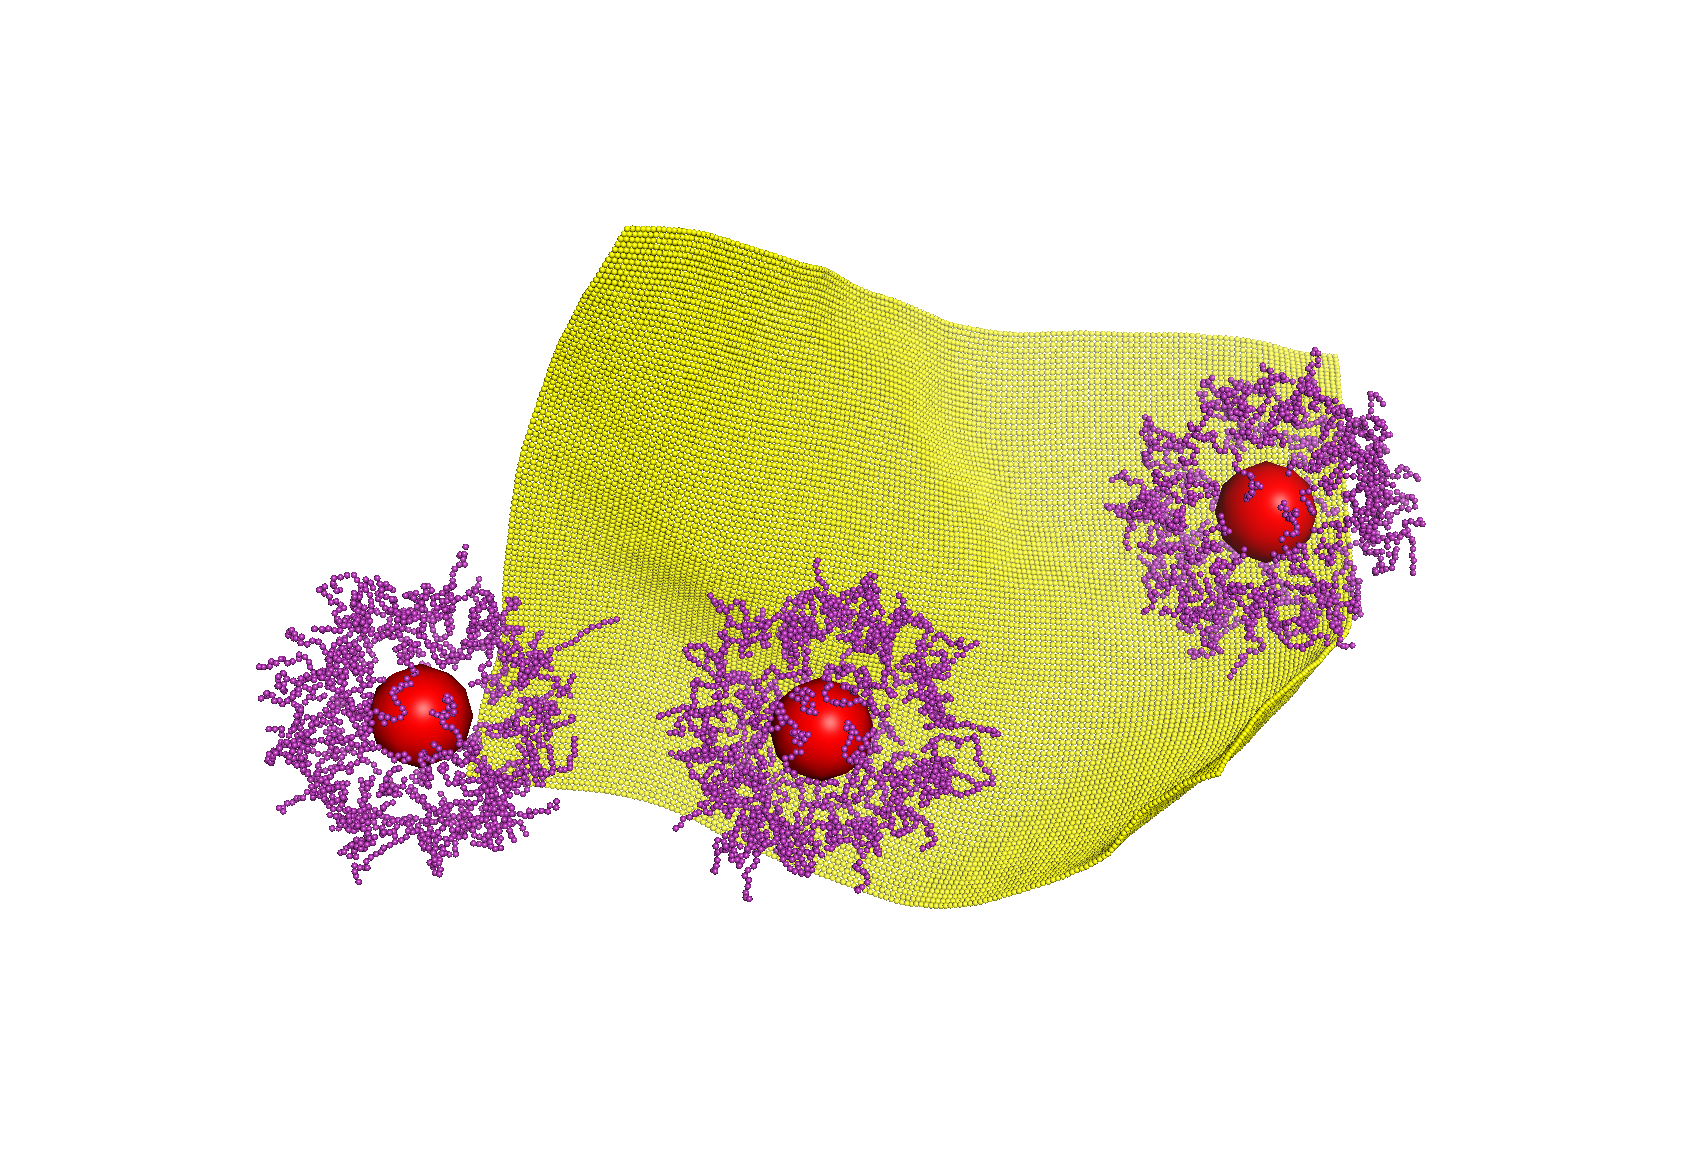
\includegraphics[width=0.7\textwidth]{80000.png}
    \caption{alkjasjj;}
    \label{fig:80000}
  \end{figure}

\end{frame}

\begin{frame}
  \frametitle{Motivation}
  \framesubtitle{ZENO/Walk-on-Spheres}

  \begin{itemize}
    \item Walk-on-Spheres accelerates Brownian Motion by jumping to a uniformly distributed point on the surface
      of a surrounding sphere
    \item The radius of the surrounding sphere is the distance of the random walker to the closest point in
      the molecule
    \item Our implementation uses \kd trees to quickly find the nearest neighbor
    \item The random access pattern of a \kd tree limits its potential for use on GPUs where memory operations
      are highly costly
  \end{itemize}

\end{frame}

\begin{frame}
  \frametitle{Specification}

  Improve performance of nearest neighbor search on \kd trees by more compactly organizing tree components
  to reduce cache misses and load instructions.

\end{frame}



%%%%%%%%%%%%%%%%%%%%%%%%%%%%%%%%%%%%%%%%
%             Background               %
%%%%%%%%%%%%%%%%%%%%%%%%%%%%%%%%%%%%%%%%

\begin{frame}
  \frametitle{\kd trees}
  \framesubtitle{Introduction}

  \begin{itemize}
    \item A \kd tree is a data structure used for partitioning $k$-dimensional space
    \item At each node, a cluster of points is partitioned by a hyperplane and the resulting
      sets of points contained in the half-spaces are passed down to the child nodes
    \item Most commonly, node hyperplanes are kept orthogonal to one coordinate axis of space
    \item Binary search trees are the one-dimensional versions of \kd trees
  \end{itemize}

\end{frame}

\begin{frame}
  \frametitle{\kd trees}
  \framesubtitle{Binary search tree}
  
  Graphic of binary search tree here
  
\end{frame}

\begin{frame}
  \frametitle{\kd trees}
  \framesubtitle{Two-dimensional \kd tree construction}
  
  Graphic of 2-d tree
  Maybe show a sequence of tree construction 
  
\end{frame}

\begin{frame}
  \frametitle{\kd trees}
  \framesubtitle{Three-dimensional \kd tree}
  
  Graphic of 3-d tree
  
\end{frame}

\begin{frame}
  \frametitle{\kd trees}
  \framesubtitle{Nearest neighbor search}

  \begin{enumerate}
    \item Given a point, $p$, rescursively move down the tree by computing its orientation relative to the 
      hyperplane $t$ by finding $p - \text{proj}_t(p)$
    \item At each node, compare the distance of the query point to the node's splitting point with the distance
      of the current nearest neighbor, if smaller, update nearest neighbor candidate
    \item Upon completion of node's recursive call, determine if distance of query point to nearest neighbor 
      candidate is larger than $\|p - \text{proj}_t(p)\|$; if it is, search the other child branch of node
  \end{enumerate}

\end{frame}

\begin{frame}
  \frametitle{\kd trees}
  \framesubtitle{Nanoflann}

  \begin{enumerate}
    \item Header only \kd tree implementation that supports k-nearest neighbor and radius search with 
      L1 or L2 metric
    \item Utilize curiously recurring template pattern and inlined functions for high performance
    \item Used for nearest neighbor search in our ZENO/Walk-on-Spheres implementation 
  \end{enumerate}

\end{frame}

%%%%%%%%%%%%%%%%%%%%%%%%%%%%%%%%%%%%%%%%
%             Limitations              %
%%%%%%%%%%%%%%%%%%%%%%%%%%%%%%%%%%%%%%%%

\begin{frame}
  \frametitle{\kd trees}
  \framesubtitle{Height and its memory limitations}

  \begin{itemize}
    \item In the best case, when the tree is balanced, the height is $O(\log n)$
    \item Each search query will require at least $O(\log n )$ pointer dereferences - very costly on graphics 
      hardware
    \item At each node we can only look ahead to one additional subspace of points
  \end{itemize}
\end{frame}

\begin{frame}
  \frametitle{\kd trees}
  \framesubtitle{Height and its memory limitations}

  \begin{itemize}
    \item Costly edge cases lead to large variance in search dereferences and time
  \end{itemize}

  Insert image showing edge case when we would have to traverse both large sides of tree
\end{frame}



\begin{frame}
  \frametitle{Flattened \kd trees}
  \framesubtitle{Introduction}

  \begin{itemize}
    \item Additional parameter $b$ specifies branching factor (i.e., number of children)
      \begin{itemize}
        \item $b$ must be a power of two
        \item Node maintains up to $b-1$ hyperplanes 
      \end{itemize}
    \item Each child accounts for a disjoint subspace of the parent's
  \end{itemize}

\end{frame}

\begin{frame}
  \frametitle{Flattened \kd trees}
  \framesubtitle{Example: $k=3$ and $b=8$}
  
  \begin{figure}
    \centering
    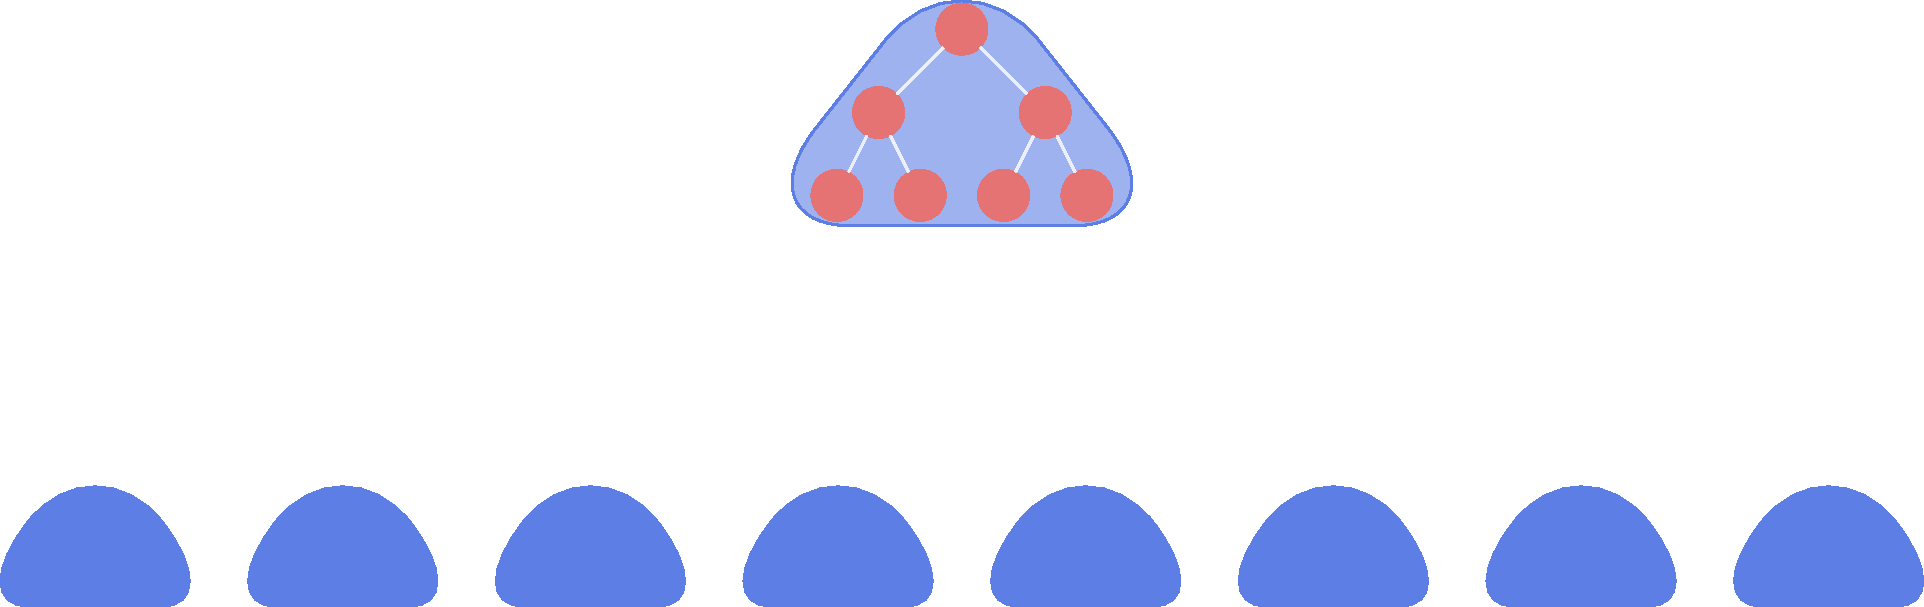
\includegraphics[width=\textwidth]{flatkdtree.pdf}
  \end{figure}

\end{frame}

\begin{frame}
  \frametitle{Flattened \kd trees}
  \framesubtitle{Advantages}

  \begin{itemize}
    \item Significantly reduced tree height
    \item More powerful look ahead to adjacent spaces when searching
    \item Greater spatial locality of tree components in memory
  \end{itemize}
\end{frame}

\begin{frame}
  \frametitle{Flattened \kd trees}
  \framesubtitle{Disadvantages}

  \begin{itemize}
    \item Additional computation per node 
      \begin{itemize}
        \item More complex path selection conditions
      \end{itemize}
    \item Greater memory footprint to fetch per node
  \end{itemize}
\end{frame}

\begin{frame}
  \frametitle{Flattened \kd trees}
  \framesubtitle{NN adjaceny check}

  \begin{figure}
    \centering
    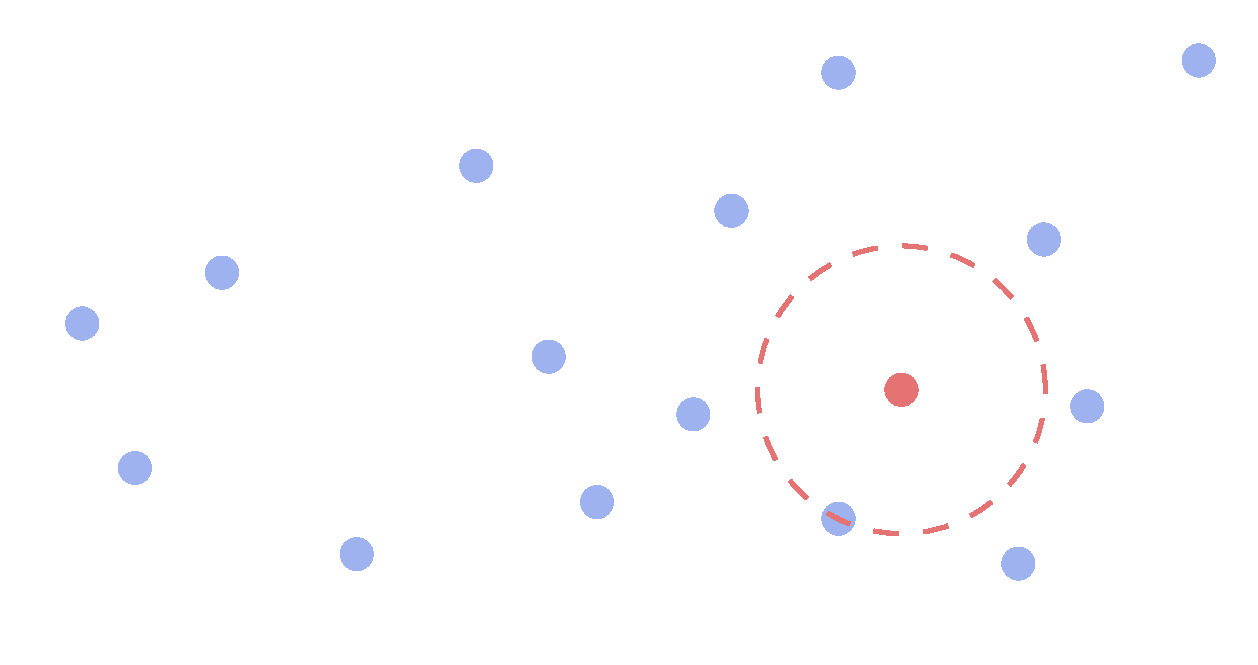
\includegraphics[width=0.85\textwidth]{nn_adjaceny_complex.pdf}
  \end{figure}

\end{frame}

\begin{frame}
  \frametitle{Flattened \kd trees}
  \framesubtitle{Initial results}

  \color{white}
  \begin{columns}[T]
    \begin{column}{0.5\textwidth}
      \vspace{-0.65cm}%
      \begin{center}
        \begin{tikzpicture}
          \centering
          \begin{axis}[
              every axis plot post/.style={/pgf/number format/fixed},
              ytick = \empty,
              ybar=5pt,
              bar width=16pt,
              axis on top,
              %xtick={2,8,16,32,64,128},
              xtick=data,
              height = 6.5cm,
              enlarge x limits=0.2,
              symbolic x coords ={2, 8, 16, 32, 64, 128},
              visualization depends on=rawy\as\rawy, % Save the unclipped values
              nodes near coords={%
                \pgfmathprintnumber{\rawy}% Print unclipped values
              },
              every node near coord/.append style={family=\DejaVu},
              y axis line style = {opacity=0},
              axis lines*=left, 
              clip=false,
              title = Pointer Dereferences,
              xlabel = Branch Factor
            ]
            %\addplot[graph-red,fill=graph-red] coordinates{(2,145)};
            \addplot[graph-blue,fill=graph-blue] coordinates {(2,145) (8, 53)
            (16, 48) (32, 56) (64, 38) (128, 33)};
          \end{axis}
        \end{tikzpicture}
      \end{center}
    \end{column}
    \begin{column}{0.5\textwidth}
      \vspace{-0.72cm}%
      \begin{center}
        \begin{tikzpicture}
          \centering
          \begin{axis}[
              every axis plot post/.style={/pgf/number format/fixed},
              ytick = \empty,
              ybar=5pt,
              bar width=16pt,
              axis on top,
              xtick=data,
              height = 6.5cm,
              enlarge x limits=0.2,
              symbolic x coords ={2, 8, 16, 32, 64, 128},
              visualization depends on=rawy\as\rawy, % Save the unclipped values
              nodes near coords={%
                \pgfmathprintnumber{\rawy}% Print unclipped values
              },
              every node near coord/.append style={family=\DejaVu},
              y axis line style = {opacity=0},
              axis lines*=left, 
              clip=false,
              title = Search Time ($\mu$s),
              xlabel = Branch Factor
            ]
            \addplot[graph-blue,fill=graph-blue] coordinates {(2,18) (8, 36)
            (16, 42) (32, 61) (64, 66) (128, 98)};
          \end{axis}
        \end{tikzpicture}
      \end{center}
    \end{column}
  \end{columns}
\end{frame}

\begin{frame}
  \frametitle{Flattened \kd trees}
  \framesubtitle{Initial results}

  \color{white}
  {\renewcommand{\arraystretch}{1.5}
  \begin{table}
    \begin{tabular}{l r r r}
      Tree & Instr. Cache Reads & Data Cache Reads & \cellcolor{graph-red}L1 Data Misses \\
      \hline \hline
      Flat \kd tree       & 77,268,111  & 31,373,726  & 314,770 \\
      Flat \kd tree (-O2) & 21,894,724  & 5,418,211   & 343,252 \\
      Nanoflann           & 53,458,672  & 23,534,300  & 284,127 \\
      \hline
    \end{tabular}
    \caption{Cache usage comparison between initial flat \kd tree and nanoflann.}
  \end{table}%
  }
\end{frame}


\end{document}
